\documentclass[12pt,a4paper,openright,twoside]{book}
\usepackage[utf8]{inputenc}
\usepackage{disi-thesis}
\usepackage{code-lstlistings}
\usepackage{notes}
\usepackage{shortcuts}
\usepackage{acronym}

\school{\unibo}
\programme{DIPARTIMENTO DI INFORMATICA – SCIENZA E INGEGNERIA

Laurea in Tecnologie dei Sistemi Informatici}
\title{Progettazione e sviluppo di un ecosistema di landing pages scalabile per una AI Transformation Company
}
\author{Francesco Santi}
\date{\today}
\subject{Progettazioe e sviluppo del software}
\supervisor{Gianluca Aguzzi}
\academicyear{2024--2025}

% Definition of acronyms
\acrodef{IoT}{Internet of Thing}
\acrodef{vm}[VM]{Virtual Machine}


\mainlinespacing{1.241} % line spacing in mainmatter, comment to default (1)

\begin{document}

% ===== FRONTESPIZIO ORIGINALE =====
\frontmatter\frontispiece

% ===== Dedica (opzionale) =====
\begin{dedication}
Dedico questo traguardo innanzitutto a Maggie che in questi anni é sempre stata al mio fianco, 
inoltre lo dedico ai miei genitori.
\end{dedication}

% ===== Introduzione (front matter, prima dell'indice) =====
% Se il tuo stile NON avesse \chapterWithoutNumber, usa la forma generica qui sotto:
\chapter*{Introduzione}
\addcontentsline{toc}{chapter}{Introduzione}

\section*{Scopo della tesi}
Lo scopo di questa tesi è documentare l'esperienza svolta presso Datapizza nel periodo compreso tra il 3 gennaio 2025 e il 20 giugno 2025, con focus sul progetto di \textbf{redesign completo delle landing pages aziendali}. Attualmente sono dipendente full-time dell'azienda nel ruolo di Software Engineer.

\section*{Il Contesto}
Datapizza è una scale-up con sede a Milano in rapida crescita che opera principalmente su quattro verticali: Tech Recruiting, Tech Community (500k+ iscritti), AI Engineering e AI Adoption. 

\section*{Ruolo e responsabilità}
Sono stato inserito nel team di prodotto come Software Engineer, con 
responsabilità prevalentemente frontend (70\%) e backend (30\%). La composizione dettagliata del team e l'organizzazione del lavoro sono approfondite nel Capitolo 6.

\section*{Il Progetto Principale}
Ho partecipato alla progettazione e sviluppo di un ecosistema di \textbf{6 landing pages specializzate}, ognuna con posizionamento chiaro, sistema di tracking avanzato e architettura scalabile:

\begin{enumerate}
  \item Home Page - Hub centrale aziendale
  \item Tech Recruiting - Matching talenti-aziende
  \item Tech Community - Community tech italiana
  \item AI Adoption - Upskilling e trasformazione
  \item AI Engineering - Sviluppo soluzioni AI
  \item Jobs Platform - Piattaforma candidati
\end{enumerate}

Questo ha permesso di: differenziare i messaggi per target specifici, implementare tracking per ottimizzare le conversioni, e abilitare marketing mirato e misurabile.

\section*{Attività complementari}
Oltre alle landing pages, ho contribuito a:
\begin{itemize}
  \item \textbf{Technical debt reduction}: standardizzazione API con 
        React Query, migrazione UI verso ShadCN, refactoring componenti, 
        miglioramento qualità del codice 
  \item \textbf{Gestionale interno}: setup architettura iniziale del 
        nuovo CRM aziendale, definizione routing e convenzioni sviluppo
  \item \textbf{Tech Recruiting}: sviluppo feature su Datapizza Jobs 
        (lato candidati) e Datapizza Company (lato aziende)
  \item \textbf{Customer support}: bug fixing, manutenzione e quality 
        assurance continuativa
\end{itemize}

Queste attività hanno arricchito l'esperienza permettendo di acquisire 
competenze trasversali e visione completa dell'ecosistema di prodotto.

% ===== Indice =====
\tableofcontents

\mainmatter

% Include dei capitoli
\chapter{Contesto aziendale}
\sloppypar
\section{Descrizione dell'azienda}
Datapizza è una scale-up innovativa con sede legale in Via Giuseppe Ripamonti 190, 20141 Milano (MI), fondata nell'ottobre 2022 con la mission di rendere l'Italia competitiva nel settore tech attraverso soluzioni avanzate e servizi mirati.

L'azienda nasce nel 2021 e ad oggi, dopo 4 anni, conta più di 60 persone e si conferma in forte crescita.

Datapizza si distingue per un approccio integrato unico nel panorama 
italiano. Questa strategia si basa su quattro verticali strategici 
complementari che operano in sinergia:


\begin{itemize}
  \item \textbf{Tech Recruiting}: connessione tra aziende e talenti tech, con oltre 50.000 professionisti registrati. Lanciato ad aprile 2023, rappresenta il ponte tra persone tecniche e aziende che vogliono essere competitive grazie alla tecnologia.
  
  \item \textbf{Tech Community}: con oltre 500.000 iscritti, costituisce la più grande community tech italiana. Punto di riferimento per notizie, tendenze e approfondimenti tecnologici, genera oltre 6 milioni di impression mensili.
  
  \item \textbf{AI Engineering}: sviluppo di agenti AI specializzati e soluzioni custom per trasformare i workflow aziendali. Include un framework proprietario (``Datapizza AI``) per l'orchestrazione di modelli, lanciato nel 2025.
  
  \item \textbf{AI Adoption}: percorsi personalizzati di trasformazione interna per potenziare la workforce aziendale. Lanciato a maggio 2023, risponde alla necessità di guidare l'adozione dell'AI in tutta l'organizzazione.
\end{itemize}

Questa struttura integrata permette all'azienda di offrire un supporto 
completo alle organizzazioni che vogliono crescere nel tech: dal 
recruiting dei talenti giusti, alla formazione delle persone, fino allo 
sviluppo di soluzioni AI personalizzate.

\section{Dimensioni e crescita}
L'azienda ha vissuto una crescita esponenziale in soli tre anni. Partita 
come community di appassionati nel 2021, è diventata società nell'ottobre 
2022 con una squadra iniziale di 10-20 persone. L'arrivo di ChatGPT nel 
novembre 2022 ha accelerato la trasformazione, portando l'AI nelle mani 
di centinaia di milioni di persone.

\medskip 
La crescita si è articolata in due fasi corrispondenti all'evoluzione del 
mercato AI. La prima fase, che copre il periodo 2023-2024, è stata 
caratterizzata dalla sperimentazione con tool AI generici. Le aziende 
iniziavano a porsi domande concrete sull'utilizzo pratico di questi 
strumenti: chi se ne doveva occupare? Come integrarli nei processi 
esistenti? Datapizza ha risposto a queste esigenze lanciando Jobs, per 
aumentare il talento tecnico interno alle organizzazioni, e AI Adoption, 
per formare le persone e favorire l'adozione consapevole della tecnologia.

\medskip 
La seconda fase, iniziata nel 2025 e tuttora in corso, vede 
l'integrazione dell'AI nei sistemi core aziendali. Non bastano più tool 
generici: serve co-progettazione con l'azienda per creare soluzioni su 
misura che rispondano a esigenze specifiche. Per questa nuova sfida, 
Datapizza ha lanciato AI Engineering con framework proprietario e 
approccio technology-first, mantenendo sempre l'essere umano al centro 
del processo decisionale.

\section{Struttura del team}
Durante il periodo documentato (3 gennaio - 20 giugno 2025), sono stato 
inserito nel team di prodotto, responsabile dello sviluppo e dell'evoluzione 
delle piattaforme software aziendali. La struttura era multidisciplinare, 
con competenze necessarie per gestire progetti complessi dall'ideazione 
al rilascio.

\medskip 
La componente design era coperta da un UX/UI Designer, che si occupava 
della progettazione dell'esperienza utente e dei wireframe, e da un 
Product Designer che definiva i requisiti di prodotto traducendo le 
esigenze di business in specifiche tecniche. Il coordinamento tecnico era 
affidato a un Tech Lead che guidava le decisioni architetturali e 
supervisionava la qualità del codice attraverso attività di code review. 
Completavano il team un AI Engineer dedicato allo sviluppo di soluzioni 
di intelligenza artificiale e integrazione dei modelli, e quattro Software 
Engineer, me compreso, focalizzati sullo sviluppo frontend e backend delle 
applicazioni.

\medskip 
Il mio ruolo è stato quello di Software Engineer con responsabilità 
prevalentemente frontend (70\%) e secondariamente backend (30\%). Questa 
suddivisione mi ha permesso di acquisire competenze approfondite sullo 
sviluppo dell'interfaccia utente e sull'esperienza d'uso, mantenendo al 
contempo una visione completa dello stack tecnologico aziendale.
\chapter{Contesto applicativo}
L'attività ha riguardato principalmente tre prodotti software:
\begin{itemize}
  \item \textbf{Datapizza Jobs} – piattaforma recruiting lato candidati;
  \item \textbf{Datapizza Company} – piattaforma recruiting lato aziende;
  \item \textbf{Datapizza Tech} – landing pages aziendali.
\end{itemize}
\chapter{Obiettivi}

\section{Obiettivi strategici e di business}
Il progetto di redesign delle landing pages aveva l'obiettivo di 
trasformare la presenza web aziendale da un'unica pagina generica a un 
ecosistema di landing specializzate, risolvendo le problematiche 
identificate nel capitolo precedente.

\paragraph{Posizionamento e differenziazione}
Un primo obiettivo strategico riguardava il posizionamento chiaro dei 
quattro verticali aziendali. Era necessario creare value proposition 
specifiche per AI Engineering, AI Adoption, Tech Recruiting e Community, 
separando nettamente la comunicazione verso aziende clienti 
business-to-business (B2B) da quella rivolta a singoli 
candidati business-to-consumer (B2C)
Questo avrebbe permesso di consolidare l'identità aziendale come 
"AI Transformation Company" attraverso messaggi mirati e coerenti per 
ciascun target.

\paragraph{Marketing data-driven e conversione}
Per abilitare decisioni basate sui dati concreti, era necessario 
implementare un sistema di tracking strutturato e conforme al regolamento 
europeo GDPR (General Data Protection Regulation) per la protezione dei 
dati personali. Gli obiettivi specifici in quest'area erano:

\begin{itemize}
  \item Implementare tracking avanzato per customer journey completi, 
        tracciando ogni interazione utente dall'arrivo sulla landing 
        fino alla conversione.
  
  \item Creare funnel di conversione misurabili per ottimizzazione 
        continua, differenziati per ciascun verticale.
  
  \item Integrare strumenti analytics (Mixpanel e Redash) per fornire 
        al team marketing dati concreti su cui basare le decisioni.
  
  \item Migliorare il conversion rate complessivo attraverso 
        l'ottimizzazione iterativa basata sui dati raccolti.
  
  \item Aumentare i lead qualificati B2B per i servizi enterprise e 
        le iscrizioni alla newsletter community.
  
  \item Ridurre il bounce rate attraverso customer journey ottimizzati 
        per ciascun tipo di utente.
\end{itemize}

\paragraph{Supporto strategia commerciale}
Le nuove landing dovevano diventare il canale primario di acquisizione 
contatti qualificati per il team sales, abilitando campagne marketing con 
misurazione accurata del ritorno sull'investimento (ROI). L'obiettivo era 
fornire visibilità completa sull'efficacia di ogni verticale e permettere 
l'allocazione ottimale del budget marketing basata su dati misurabili.

\section{Obiettivi tecnici}
Gli obiettivi tecnici erano orientati a costruire un'infrastruttura 
solida, performante e scalabile per supportare gli obiettivi di business.

\subsection{Architettura e scalabilità}
L'obiettivo architetturale principale era costruire un sistema frontend 
moderno basato su un design system modulare. La scelta di ShadCN UI e 
Tailwind CSS come fondamenta permetteva di creare componenti riutilizzabili 
e mantenere consistenza visiva tra tutte le landing. L'architettura doveva 
supportare il multilingua attraverso percorsi dedicati (/it/ e /en/) e 
garantire la scalabilità futura: ogni nuova landing page doveva poter 
riutilizzare la maggior parte del codice esistente, riducendo 
significativamente i tempi di sviluppo per futuri verticali.

\subsection{Performance e user experience}
Dal punto di vista delle performance, l'obiettivo era garantire 
caricamenti rapidi attraverso tecniche di ottimizzazione come code 
splitting, lazy loading e compressione delle immagini. L'esperienza 
doveva essere fluida su tutti i dispositivi (desktop, tablet, mobile). 

Particolare attenzione era richiesta per l'accessibilità: conformità 
agli standard WCAG 2.1 (Web Content Accessibility Guidelines)
per supportare utenti con disabilità attraverso screen reader, navigazione 
da tastiera e contrasto colori adeguato. Questi standard internazionali 
definiscono criteri tecnici per rendere i contenuti web accessibili a 
persone con diverse tipologie di disabilità visive, uditive, motorie e 
cognitive.

\subsection{Tracking e analytics}
L'obiettivo sul fronte analytics era integrare Mixpanel con una event 
taxonomy strutturata per categorizzare i comportamenti utente in tre 
categorie principali: page view (visualizzazioni), interaction 
(interazioni con elementi della pagina) e conversion (azioni di valore 
come submit form o iscrizione newsletter). Ogni verticale doveva avere 
funnel di conversione specifici e misurabili, differenziati per tipo di 
utente (B2B enterprise, B2C candidati, Community). La conformità GDPR 
era un requisito non negoziabile, da garantire attraverso consenso 
esplicito ai cookie, anonimizzazione degli indirizzi IP e gestione 
delle preferenze privacy degli utenti.
\chapter{Tecnologie}

\section{Stack tecnologico landing pages}
Il progetto di redesign delle landing pages si basa su uno stack moderno 
orientato a performance, SEO e developer experience. Le scelte tecnologiche 
sono state guidate dalla necessità di garantire caricamenti rapidi, 
indicizzazione ottimale sui motori di ricerca e scalabilità futura.

\subsection{Frontend}

Il framework principale è Next.js 15, che si basa su React 19 e TypeScript 
5.7. Queste tecnologie erano già in uso nel progetto precedente e sono 
state mantenute durante il redesign per coerenza con l'intero ecosistema 
tecnologico aziendale.

\paragraph{React 19}
React è la libreria JavaScript per costruire interfacce utente component-based, 
utilizzata in tutti i principali prodotti Datapizza (Jobs, Company, gestionale 
interno). Questa coerenza tecnologica garantisce riuso del codice, competenze 
consolidate del team e facilita l'inserimento di nuovi sviluppatori. L'approccio 
component-based permette di costruire interfacce modulari suddividendo 
l'interfaccia in componenti indipendenti e riutilizzabili, facilitando la 
manutenzione e la scalabilità del codice.

\paragraph{TypeScript 5.7}
A supporto di React è stato adottato TypeScript 5.7, un superset di 
JavaScript che aggiunge type safety statico, ormai standard per applicazioni 
moderne in contesti production. L'adozione di TypeScript riduce significativamente 
la probabilità di errori in produzione grazie al type checking in fase di 
sviluppo: errori comuni come accesso a proprietà inesistenti o passaggio di 
parametri errati vengono intercettati dal compilatore prima del deployment. 
In un contesto production come le landing pages, dove errori critici impattano 
direttamente le conversioni, TypeScript è fondamentale per garantire affidabilità.

TypeScript migliora significativamente il lavoro in team rendendo il codice più 
strutturato e auto-documentato. L'autocompletion intelligente negli IDE accelera 
lo sviluppo, mentre il supporto al refactoring permette modifiche strutturali 
sicure, riducendo il tempo di apprendimento per nuovi sviluppatori.

\paragraph{Next.js 15}
Next.js è un framework React ampiamente adottato per lo sviluppo di applicazioni 
production-ready, fornendo funzionalità avanzate di rendering e ottimizzazione. 
La scelta di Next.js rispetto a React standalone si basa su tre vantaggi 
fondamentali per il progetto.

Il rendering ibrido combina diverse strategie di generazione delle pagine: 
Server-Side Rendering (SSR) per generare HTML dinamico ad ogni richiesta, 
Static Site Generation (SSG) per pre-generare pagine statiche in fase di build, 
e Incremental Static Regeneration (ISR) che estende SSG permettendo 
l'aggiornamento incrementale di contenuti statici senza rigenerare l'intero 
sito. Questo approccio ottimizza sia i tempi di caricamento che la freschezza 
dei contenuti.

Il SEO nativo garantisce che i motori di ricerca ricevano HTML completo 
server-side, fondamentale per indicizzazione efficace e traffico organico. 
Il code splitting automatico suddivide il codice in bundle separati per 
ogni route, caricando solo lo stretto necessario per la pagina corrente 
e riducendo il tempo di primo caricamento.

Next.js supporta nativamente il routing internazionalizzato, esteso in questo 
progetto tramite la libreria next-intl per gestire i percorsi localizzati 
(/it/ e /en/). Il componente next/image ottimizza automaticamente le immagini: 
conversione in formato moderno (WebP/AVIF), caricamento differito quando 
l'immagine entra nel viewport (lazy loading), e generazione di varianti 
responsive per adattarsi alle dimensioni del dispositivo, riducendo il peso 
complessivo mantenendo qualità visiva.

\subsection{Styling e UI}

Per garantire coerenza visiva con l'identità aziendale, il sistema di styling 
si basa su Tailwind CSS integrato con la component library ShadCN UI.

Tailwind CSS è un framework CSS utility-first (approccio basato su classi 
utilitarie) che permette di costruire interfacce applicando classi predefinite 
direttamente nel markup HTML, eliminando la necessità di scrivere file CSS 
separati. A differenza dei framework tradizionali basati su componenti 
pre-stilizzati (come Bootstrap), Tailwind fornisce classi atomiche di basso 
livello che compongono lo stile finale. Durante la fase di build, solo le 
classi effettivamente utilizzate vengono compilate nel CSS finale, riducendo 
drasticamente le dimensioni del bundle e garantendo tempi di caricamento ridotti.

ShadCN UI completa l'infrastruttura di styling fornendo componenti accessibili 
basati sulle primitive Radix UI, con conformità nativa agli standard WCAG 2.1 
livello AA. A differenza delle librerie tradizionali, ShadCN UI genera i 
componenti direttamente nel progetto tramite command-line interface, garantendo 
pieno controllo sul codice senza dipendenze esterne rigide. L'integrazione con 
Tailwind permette di stilizzare i componenti con utility classes, combinando 
accessibilità e flessibilità di design.

\subsection{Librerie complementari}

Per animazioni e interattività avanzate, il progetto utilizza Framer Motion per 
animazioni fluide nelle sezioni principali (Hero sections) e Three.js con React 
Three Fiber per visualizzazioni 3D sulla landing AI Engineering. La gestione dei 
form si basa su React Hook Form per performance ottimali e Zod per validazione 
dello schema dati con supporto TypeScript integrato sui form di acquisizione lead.

Il tracking degli eventi utente è gestito tramite Mixpanel, piattaforma di 
product analytics che permette di tracciare interazioni personalizzate e 
costruire funnel di conversione differenziati per verticale. A differenza di 
strumenti generici come Google Analytics, Mixpanel offre granularità event-based: 
ogni interazione utente (click su call-to-action, scroll della pagina, apertura 
form) viene tracciata come evento discreto, permettendo analisi dettagliate del 
customer journey. L'SDK Mixpanel viene inizializzato lato client solo dopo 
consenso esplicito dell'utente tramite cookie banner, in conformità al GDPR 
mediante anonimizzazione degli indirizzi IP e gestione delle preferenze di 
privacy.

\subsection{Backend per dati dinamici}

Alcune funzionalità delle landing pages richiedono elaborazioni lato server 
che il frontend non può gestire autonomamente, come la validazione sicura dei 
form, l'integrazione con servizi esterni e l'accesso al database aziendale.

Il backend è condiviso tra tutti i prodotti Datapizza: oltre alle landing pages, 
serve le applicazioni Jobs (lato candidati), Company (lato aziende) e il CRM 
interno. Questa architettura unificata consente una manutenzione centralizzata 
e garantisce consistenza dei dati tra piattaforme.

\paragraph{Django e Python}
Il backend si basa su Django, framework web scritto in Python. Python è un 
linguaggio di programmazione ad alto livello, apprezzato per la sua semplicità 
sintattica e il vasto ecosistema di librerie, particolarmente ricco nell'ambito 
data science e intelligenza artificiale. Django fornisce un'architettura robusta 
per costruire API REST in modo rapido e sicuro, con strumenti integrati per 
autenticazione, gestione database e validazione dati.

\paragraph{PostgreSQL}
Il database utilizzato è PostgreSQL, sistema di gestione database relazionale 
open-source. PostgreSQL organizza i dati in tabelle strutturate collegate tra 
loro tramite relazioni, garantendo integrità referenziale e consistenza. Nel 
contesto del progetto, PostgreSQL gestisce le opportunità lavorative visualizzate 
sulla Jobs Platform, i dati degli utenti registrati e le informazioni aziendali.

\paragraph{Funzionalità principali}
Il backend gestisce diverse integrazioni critiche per il funzionamento delle 
landing pages. I form di contatto passano attraverso validazione lato server 
per prevenire input malevoli e garantire che solo dati validi raggiungano il 
database. L'integrazione con Customer.io, piattaforma di email automation, 
gestisce le iscrizioni alla newsletter "Commit" e l'invio di comunicazioni 
personalizzate agli oltre 500.000 iscritti della community. Il sistema fornisce 
inoltre API per il recupero in tempo reale delle opportunità lavorative 
visualizzate sulla Jobs Platform.

Deployato su infrastruttura cloud AWS, lo stack backend completo si basa su 
Django 4.x, PostgreSQL 15 e Python 3.9, per garantire scalabilità e disponibilità. 
L'infrastruttura di deployment su AWS è dettagliata nel Capitolo 7, mentre 
la Figura~\ref{fig:stack-landing} illustra l'architettura applicativa 
complessiva delle landing pages.

\begin{figure}[h!]
    \centering
    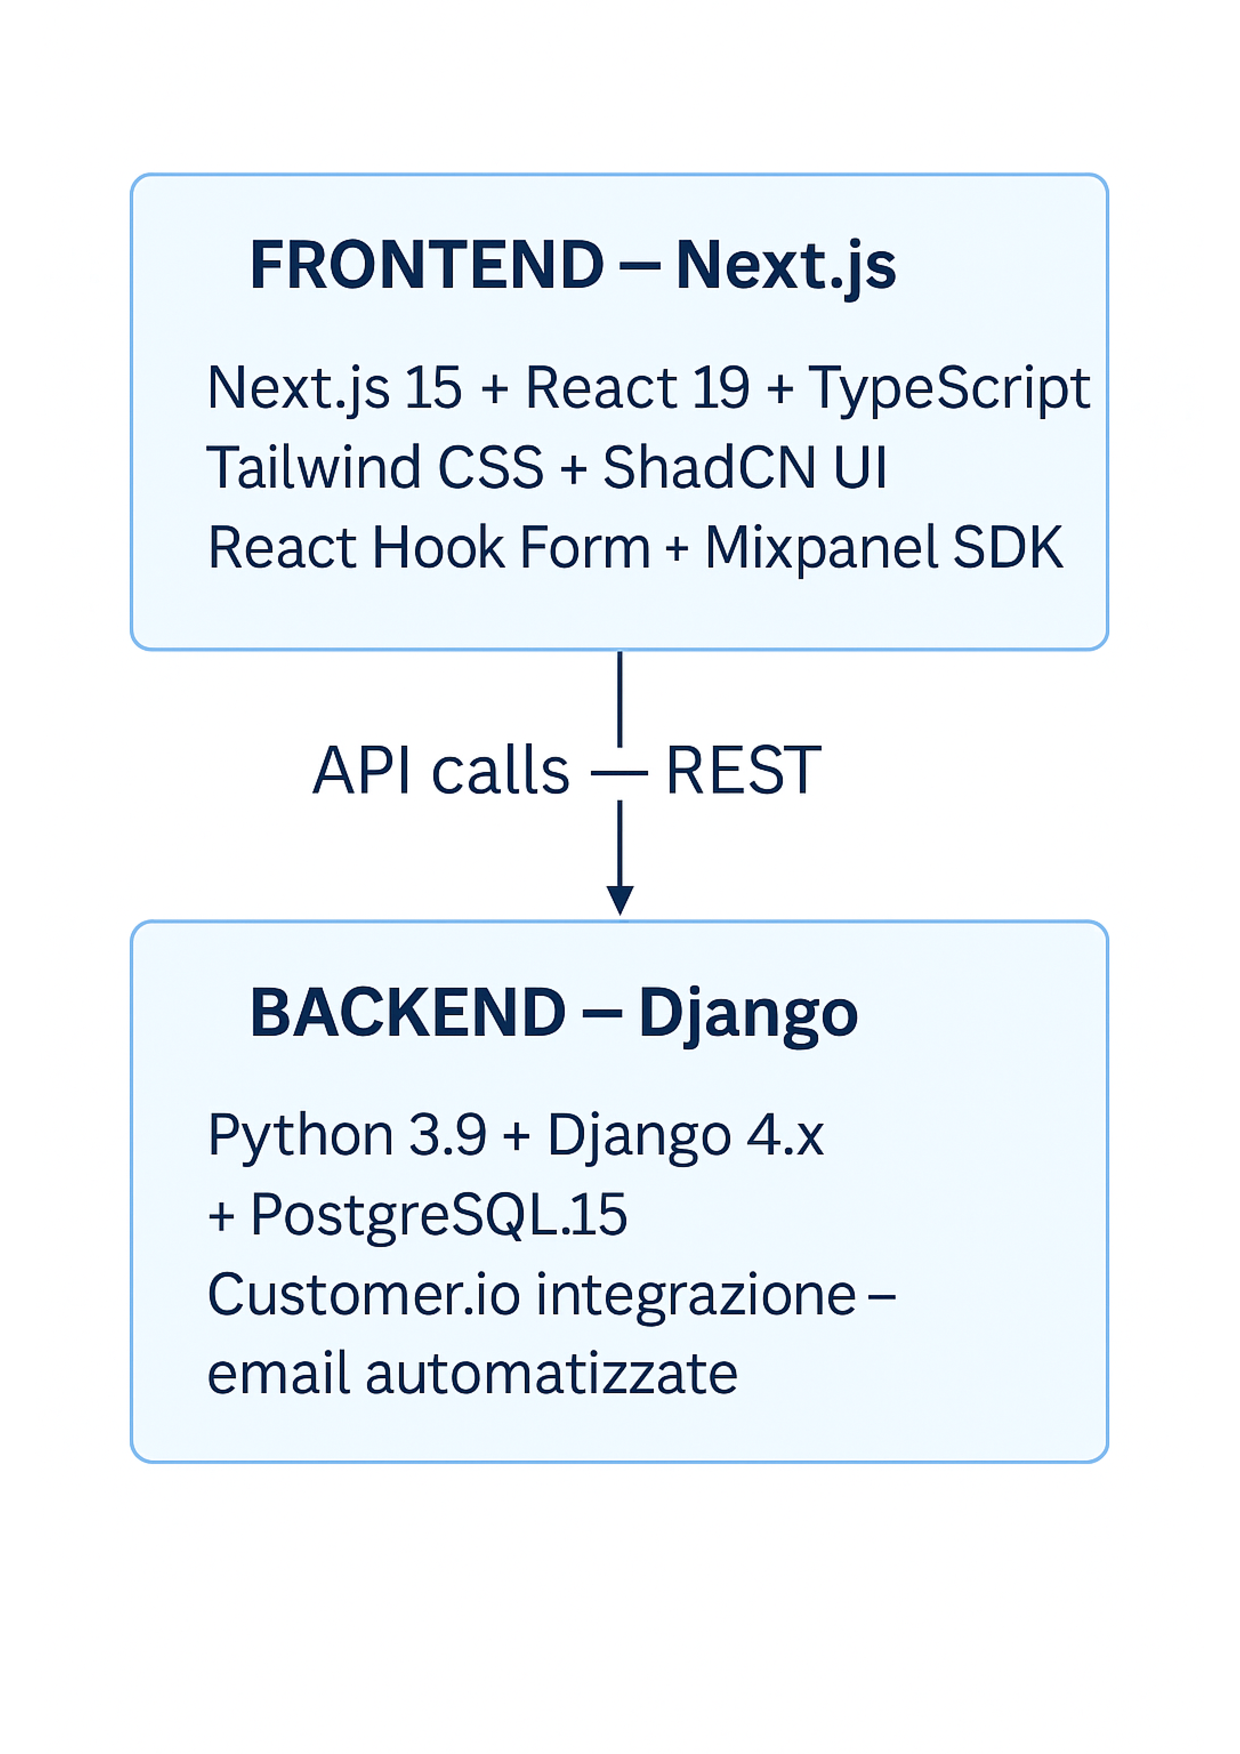
\includegraphics[width=0.52\textwidth]{chapters/figures/stack2.pdf}
    \caption{Architettura applicativa delle landing pages che mostra 
    l'interazione tra frontend e backend 
 tramite API REST.}
    \label{fig:stack-landing}
\end{figure}

\clearpage

\section{Stack tecnologico aziendale}

L'ecosistema Datapizza (Jobs, Company, gestionale, landing pages) condivide 
uno stack unificato per garantire coerenza tecnologica e riutilizzo di competenze 
tra prodotti. La Tabella~\ref{tab:stack-aziendale} fornisce una panoramica 
completa delle tecnologie adottate a livello aziendale.

\begin{table}[h]
\centering
\caption{Stack tecnologico aziendale}
\label{tab:stack-aziendale}
\begin{tabular}{|l|l|p{6.5cm}|}
\hline
\textbf{Layer} & \textbf{Tecnologie} & \textbf{Note} \\
\hline
Frontend & React 19, TypeScript 5.7 & Base comune tutti i prodotti \\
\hline
Frontend & React Query & State management server-side \\
\hline
Frontend & TanStack Router & Routing type-safe (CRM) \\
\hline
Backend & Django 4.x, PostgreSQL 15 & Stack verticale Python \\
\hline
Infrastructure & AWS (eu-south-1) & Cloud provider \\
\hline
Infrastructure & Docker, AWS ECR & Containerizzazione \\
\hline
Infrastructure & S3, CloudFront & Storage e distribuzione globale \\
\hline
Infrastructure & Lambda & Integrazioni AI serverless \\
\hline
Tools & Mixpanel & Analytics GDPR-compliant \\
\hline
Tools & Customer.io & Email automation (500k+ iscritti) \\
\hline
\end{tabular}
\end{table}

\section{Development tools e workflow}

Il team utilizza una suite integrata di strumenti per garantire efficienza, 
qualità del codice e collaborazione efficace. La Tabella~\ref{tab:dev-tools} 
riassume le principali tecnologie adottate.

\clearpage
\begin{table}[h]
\centering
\caption{Strumenti di sviluppo e workflow}
\label{tab:dev-tools}
\begin{tabular}{|l|l|p{6cm}|}
\hline
\textbf{Categoria} & \textbf{Tecnologia} & \textbf{Utilizzo} \\
\hline
IDE & VS Code + Cursor AI & Editor principale con AI assistance \\
\hline
Version Control & GitLab self-hosted & Repository privato, Merge Request \\
\hline
Project Management & Jira & Task tracking, sprint planning \\
\hline
Deployment & Docker + AWS ECR & Containerizzazione e registry \\
\hline
Communication & Discord, Google Meet & Daily standup, sync team \\
\hline
Documentation & Notion & Knowledge base, onboarding \\
\hline
\end{tabular}
\end{table}

Il workflow di sviluppo segue approccio Agile con sprint bisettimanali. Il 
codice viene sviluppato su branch Git dedicati per ogni nuova funzionalità 
(feature branches), e ogni modifica richiede Merge Request su GitLab con 
revisione del codice (code review) obbligatoria da parte di almeno un 
collega prima dell'integrazione nel branch principale. Jira traccia le user 
stories con stima della complessità in story points, mentre grafici di 
avanzamento (burndown charts) monitorano il progresso di ogni sprint. La 
documentazione tecnica è centralizzata su Notion per garantire accessibilità 
rapida a tutto il team.
\chapter{Progettazione}

La fase di progettazione ha avuto l'obiettivo di tradurre i requisiti individuati
nei capitoli precedenti in un'architettura scalabile, accessibile e coerente con
l'identità aziendale. In questa sezione vengono presentate le decisioni
architetturali chiave, il processo metodologico adottato e l'organizzazione
dell'ecosistema di landing pages.

\section{Decisioni architetturali}
Il punto di partenza era una landing page unica, insufficiente per comunicare i
diversi verticali aziendali e raccogliere dati utili a livello di marketing. La
progettazione ha quindi introdotto tre scelte fondamentali:

\begin{itemize}
  \item \textbf{Architettura multi-landing}: adozione di un monorepo Next.js con sei
  route dedicate (/it/, /it/tech-recruiting/, /it/ai-adoption/, etc.), così da garantire 
  posizionamento SEO ottimale, riuso di componenti comuni e semplicità di manutenzione. 
  
  \item \textbf{Strategia di rendering}: adozione di Static Site Generation (SSG) 
  con Incremental Static Regeneration (ISR, revalidation 1 ora), che consente di 
  bilanciare performance, costi infrastruttura e 
  necessità di aggiornamento contenuti. Scelta motivata da requisiti performance 
  critici per conversioni e traffico organico, con HTML statico servito da CDN 
  per crawler Google.
  
  \item \textbf{Design system condiviso}: definizione di una libreria di componenti 
  accessibili basata su ShadCN UI (Radix UI primitives) e Tailwind CSS, costruita 
  su linee guida visive aziendali. Garantisce accessibilità WCAG 2.1 AA nativa, 
  customizzazione completa e riutilizzo del codice UI tra le landing.
\end{itemize}

\section{Metodologia di progettazione e collaborazione} Il progetto di redesign è stato organizzato come una \textbf{macro-release trimestrale},
considerata strategica per l'azienda. La fase di progettazione non si è limitata
alla definizione di scelte tecniche, ma ha previsto un percorso strutturato di
analisi, collaborazione e validazione:

\begin{itemize}
  \item \textbf{Analisi iniziale}: revisione delle soluzioni esistenti e
  identificazione dei pattern da mantenere o eliminare.
  \item \textbf{Collaborazione interfunzionale}: raccolta dei requisiti in
  incontri con i team di prodotto, marketing e design, così da garantire
  allineamento tra esigenze di business e soluzioni tecniche.
  \item \textbf{Iterazioni e feedback}: rilascio preliminare delle nuove landing
  a un gruppo ristretto di stakeholder interni, con raccolta feedback e successive
  ottimizzazioni.
  \item \textbf{Approccio Agile}: gestione del lavoro in sprint bisettimanali,
  con daily standup, retrospettive e momenti di confronto dedicati alla revisione
  della qualità.
  \item \textbf{Progettazione responsive}: attenzione fin dall'inizio alle tre
  principali dimensioni di visualizzazione (desktop, tablet e mobile), per
  garantire una user experience coerente e ottimizzata.
\end{itemize}

Questa metodologia ha consentito di ridurre i rischi, migliorare la qualità
finale e assicurare che le landing rispondessero realmente ai bisogni degli utenti
e dell'azienda.

\section{Processo di design e design system}
Il design system è stato sviluppato in stretta collaborazione con il team UX/UI,
a partire da wireframe validati con il product team fino a mockup
high-fidelity realizzati in Figma. Il processo ha incluso:

\begin{itemize}
  \item definizione di design tokens comuni (colori, tipografia, spaziatura),
  condivisi tra Figma e configurazioni Tailwind CSS di progetto;
  \item creazione di componenti modulari con varianti responsive, per garantire 
  consistenza visiva e riutilizzo tra le 6 landing pages;
\end{itemize}

L'architettura componenti ha permesso di standardizzare elementi ricorrenti garantendo il riutilizzo di molto del codice UI tra le diverse landing.

Questo approccio ha permesso di ridurre i tempi di sviluppo, garantire coerenza tra design e implementazione e abilitare una rapida iterazione.

\section{Architettura delle landing pages}
L'ecosistema è stato progettato con una struttura comune di base (\textit{navbar}, 
\textit{footer}) e con personalizzazioni specifiche per ciascun verticale. 
Ogni landing è stata progettata con tone of voice e UX mirati:

\begin{itemize}
  \item \textbf{Home Page} (/it/): hub centrale con overview dei 4 verticali e 
  routing intelligente verso servizi specifici. Target: visitatori generici.
  
  \item \textbf{Tech Recruiting} (/it/tech-recruiting/): tone of voice 
  consulenziale B2B, layout pulito, form di contatto avanzati con campi aziendali, 
  CTA orientate a demo ("Richiedi demo", "Contatta team"). Target: aziende in 
  cerca di talenti tech.
  
  \item \textbf{Tech Community} (/it/tech-community/): linguaggio informale, 
  elementi visuali orientati alla cultura developer, CTA engagement per newsletter 
  "Commit", social proof con 500k+ iscritti. Target: developer e tech enthusiast.
  
  \item \textbf{AI Adoption} (/it/ai-adoption/): tone professionale B2B enterprise, 
  focus upskilling organizzativo e trasformazione interna, case studies aziendali, 
  CTA consulenza personalizzata. Target: HR e management.
  
  \item \textbf{AI Engineering} (/it/ai-engineering/): showcase framework 
  proprietario "Datapizza AI" con gallery progetti (Copiloti Sales/HR/Legal/Customer), 
  CTA demo tecnica. Target: CTO e IT Decision Makers.
  
  \item \textbf{Jobs Platform} (/jobs/): stile diretto e colorato B2C, 
  call-to-action immediate ("Cerca lavoro", "Candidati ora"), esperienza 
  mobile-first, trasparenza salary con RAL sempre visibile, Tech Buddy matching 
  e zero ghosting policy. Target: candidati in cerca di opportunità tech.
\end{itemize}

\begin{figure}[h!]
    \centering
    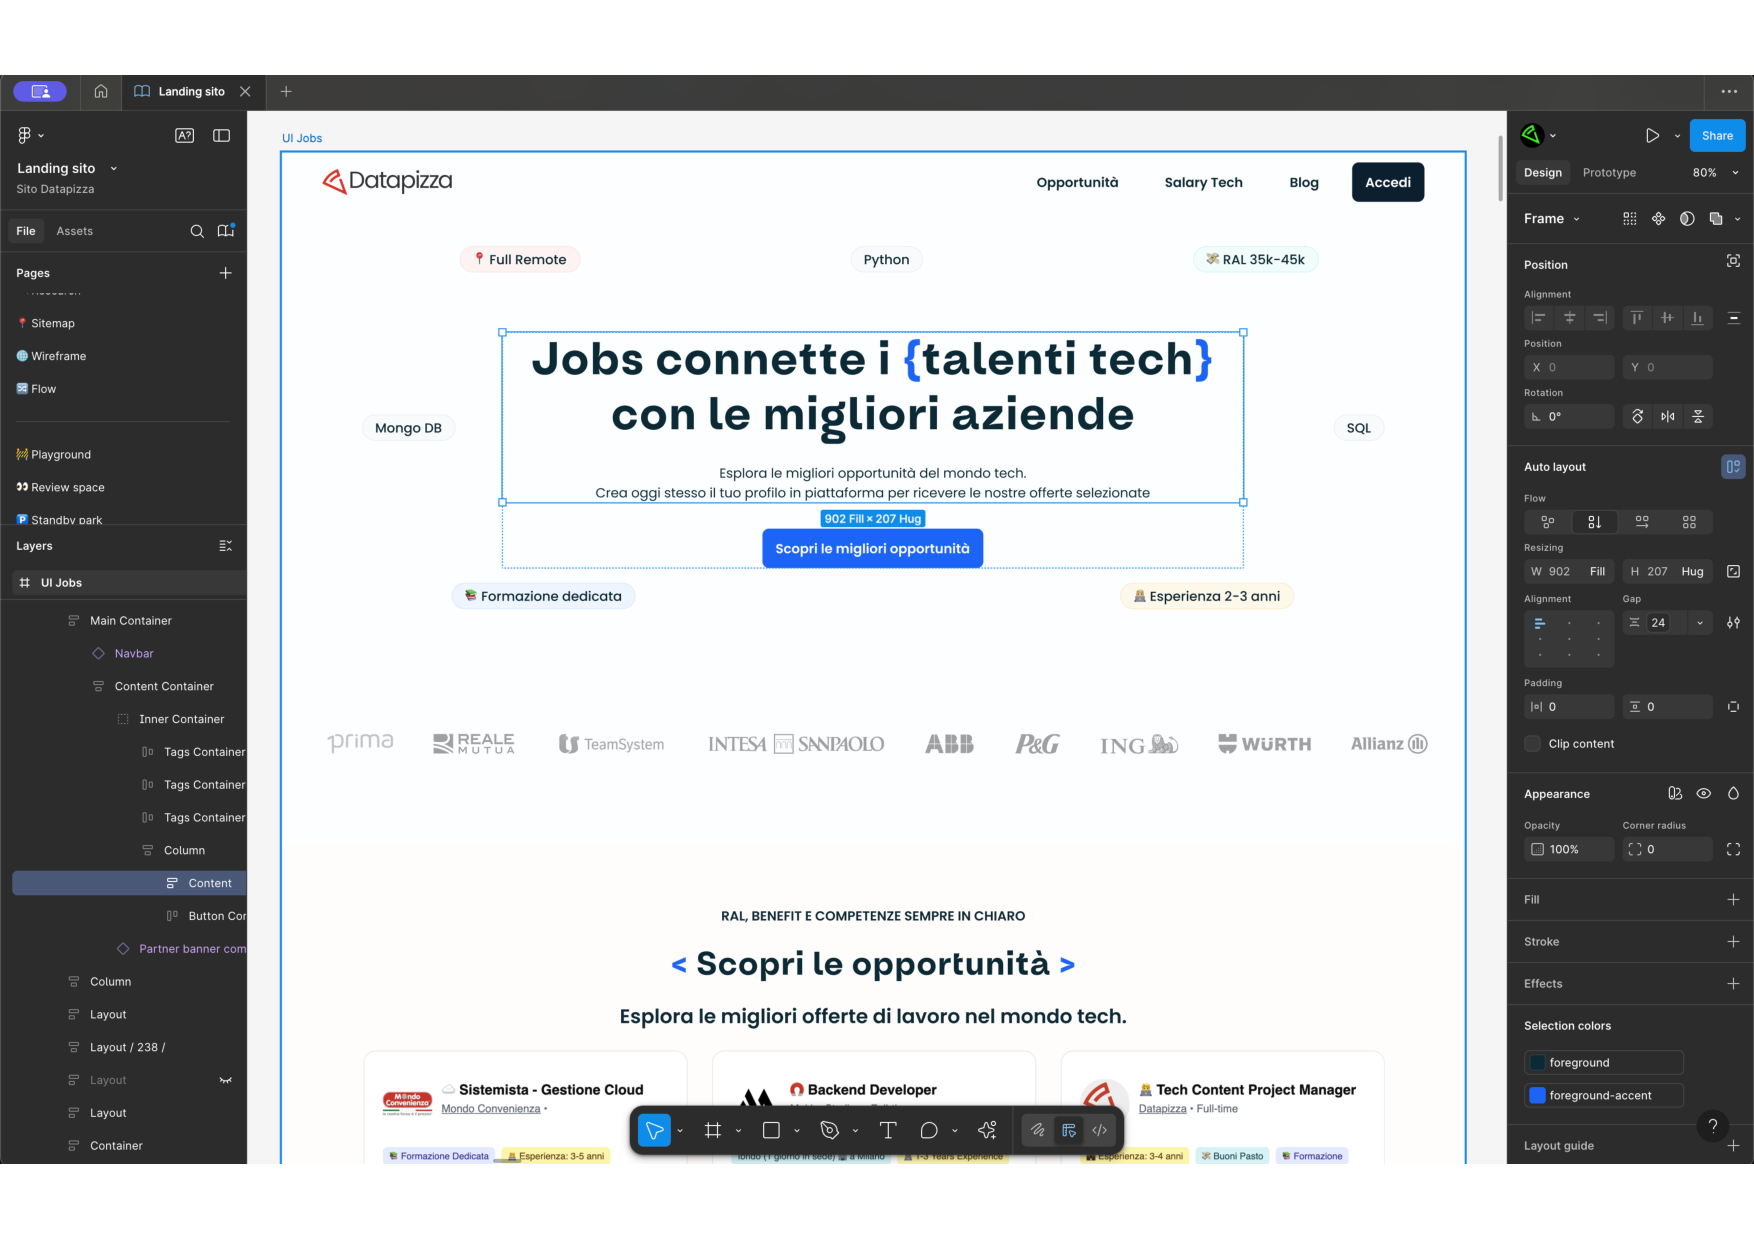
\includegraphics[width=1.1\textwidth]{chapters/figures/mockup.pdf}
    \caption{Schermata mockup desktop jobs.}
    \label{fig:refactoring}
\end{figure}

\begin{figure}[h!]
    \centering
    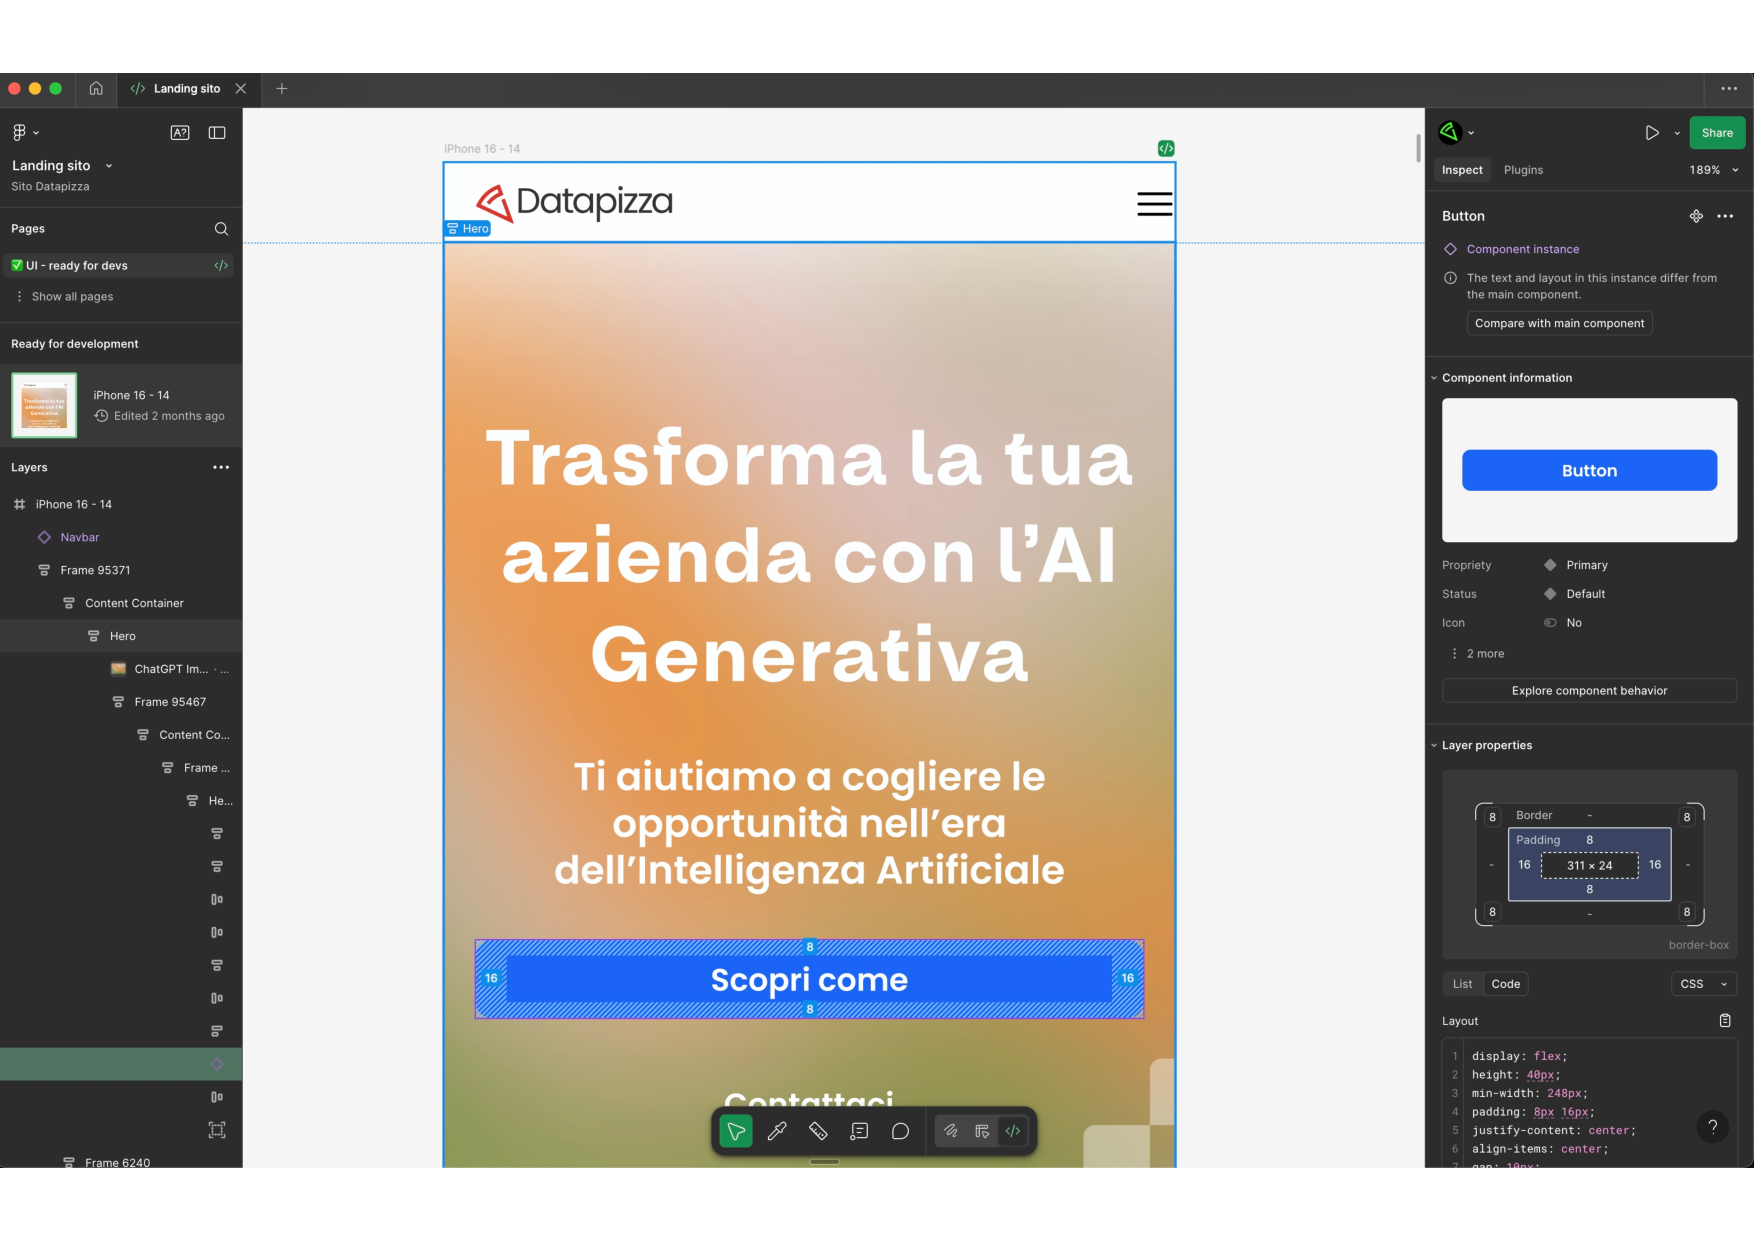
\includegraphics[width=1.1\textwidth]{chapters/figures/mockup2.pdf}
    \caption{Schermata mockup mobile AI eng.}
    \label{fig:refactoring}
\end{figure}

\section{Tracking e misurabilità}
Il sistema di tracking è stato progettato per migliorare l'implementazione 
precedentemente presente, supportando funnel di conversione specifici per ogni 
verticale. L'integrazione con Mixpanel consente di tracciare page view, 
interazioni e conversioni con granularità maggiore rispetto alla soluzione unica 
precedente.

\subsection{Event taxonomy e funnel}
L'architettura tracking implementa una tassonomia strutturata di eventi:
\begin{itemize}
  \item \textbf{Page events}: page\_view, landing\_loaded
  \item \textbf{Interaction events}: cta\_clicked, scroll\_depth, section\_viewed
  \item \textbf{Conversion events}: form\_submitted, newsletter\_signup
\end{itemize}

Il tracking permette di analizzare funnel di conversione differenziati per verticale:
\begin{itemize}
  \item \textbf{B2B}: landing\_view → cta\_click → form\_view → form\_submit
  \item \textbf{B2C Jobs}: landing\_view → search\_used → position\_click → application\_start
  \item \textbf{Community}: landing\_view → scroll\_50\% → newsletter\_click → newsletter\_submit
\end{itemize}

Questa segmentazione consente analisi specifiche per ottimizzazione delle 
conversioni e identificazione dei punti di drop-off nel customer journey.

\subsection{GDPR compliance}
Particolare attenzione è stata data alla conformità normativa europea con 
approccio privacy-by-design: consenso esplicito tramite cookie banner prima 
di inizializzazione Mixpanel, anonimizzazione automatica degli indirizzi IP 
e gestione opt-out utente.

\bigskip
In sintesi, la progettazione ha permesso di definire una base solida dal punto di
vista tecnico e metodologico, con decisioni architetturali motivate e framework 
scalabile, che ha guidato lo sviluppo e il dispiegamento presentati nei capitoli 
successivi.
\chapter{Sviluppo}

\section{Processo di sviluppo}
Lo sviluppo delle landing pages è stato organizzato con un approccio
iterativo basato su sprint bisettimanali. Ogni sprint prevedeva
pianificazione delle priorità, sviluppo incrementale, revisione del
codice e demo finale con stakeholder per raccogliere feedback.  
Il workflow ha incluso code review obbligatoria su ogni Pull Request,
testing continuo su ambiente \textit{staging} e rilascio progressivo
per singola landing.

\section{Fasi di implementazione}
Il progetto è stato articolato in quattro fasi principali:

\begin{itemize}
  \item \textbf{Fase 1 – Architettura e design system}: setup del progetto
  Next.js con App Router, configurazione multilingua e definizione del design
  system base con Tailwind e ShadCN.
  \item \textbf{Fase 2 – Sviluppo landing pages}: implementazione progressiva
  delle sei landing, a partire dalla Home Page (validazione del design system) fino alla Jobs Platform.
  \item \textbf{Fase 3 – Tracking e ottimizzazione}: integrazione completa di
  Mixpanel, funnel di conversione per verticale, cookie consent GDPR e
  ottimizzazioni SEO e performance.
  \item \textbf{Fase 4 – Deploy e monitoring}: rilascio graduale in produzione,
  monitoraggio in tempo reale con Mixpanel e Vercel Analytics, e documentazione finale.
\end{itemize}

\section{Sviluppo delle landing}
Le landing sono state sviluppate seguendo priorità strategiche. La
\textbf{Home Page} è stata la prima, hub centrale con routing verso i verticali
e social proof aziendali.  
Sono seguite le pagine \textbf{Tech Recruiting} e \textbf{Community}, rispettivamente orientate a lead generation B2B e alla crescita della community.  
Successivamente sono state realizzate \textbf{AI Adoption} e \textbf{AI Engineering}, focalizzate sui servizi enterprise, e infine la \textbf{Jobs Platform}, progettata mobile–first con ricerca avanzata e trasparenza salariale.  

\section{Implementazione architettura}
Come progettato nel capitolo precedente, l'implementazione ha seguito le decisioni 
architetturali chiave: monorepo Next.js con 6 route dedicate, SSG con ISR per 
performance ottimali, e design system basato su ShadCN UI.

Dal punto di vista tecnico, lo sviluppo ha previsto tre aree principali:

\textbf{Architettura componenti} – è stata realizzata una libreria di componenti 
riutilizzabili con TypeScript per garantire consistenza e riuso tra le 6 landing pages.

\textbf{Routing e rendering} – le landing sono state generate staticamente
(SSG) con revalidazione oraria (ISR), con gestione automatica di meta tags e
sitemap per l'ottimizzazione SEO.  

\textbf{Tracking e compliance} – l'SDK di Mixpanel è stato integrato con 
inizializzazione condizionale dopo consenso esplicito e anonimizzazione IP 
per conformità GDPR.

\section{Sfide affrontate e soluzioni}
Durante lo sviluppo sono emerse diverse difficoltà tecniche risolte con 
soluzioni specifiche:

\textbf{Cross-browser compatibility} – Safari mostrava incompatibilità con 
regex JavaScript per validazione form. La soluzione è stata implementare 
validazione alternativa con Zod schema per garantire funzionamento uniforme 
su tutti i browser.

\textbf{Performance con contenuti ricchi} – la landing AI Engineering, con
gallery e componenti interattivi, presentava tempi di caricamento elevati. 
Ottimizzazione immagini (WebP), lazy loading e dynamic import hanno migliorato 
significativamente le performance, raggiungendo i target Lighthouse prefissati.  

\textbf{Bundle optimization} – il bundle iniziale risultava eccessivamente 
pesante. L'implementazione di code splitting automatico per route e dynamic 
import per componenti pesanti ha ridotto il payload iniziale, migliorando 
First Contentful Paint.

\textbf{Tracking inconsistente} – eventi Mixpanel non venivano tracciati 
correttamente su dispositivi iOS in modalità Private Browsing. Implementazione 
graceful degradation e fallback per tracking senza localStorage ha risolto 
la problematica.

\section{Esempio implementazione}
Segue un esempio di implementazione tecnica significativa per il progetto:

\begin{lstlisting}[language=JavaScript, caption=Custom hook per tracking]
// hooks/use-mixpanel.ts
const track = useCallback((event: string, properties?: Record<string, any>) => {
  // Implementation details
}, []);
\end{lstlisting}

Questo esempio illustra l'approccio adottato per garantire tracking consistente 
e GDPR-compliant attraverso hook personalizzati riutilizzabili.

\section{Testing e qualità}
Il progetto è stato sottoposto a una strategia di quality assurance che ha
incluso test manuali su staging, validazione cross-browser e responsive,
verifica accessibilità WCAG 2.1 AA, monitoraggio performance con Lighthouse CI e
controlli regressivi su ogni landing.  

La qualità del codice è stata mantenuta tramite ESLint, Prettier, typing
rigoroso con TypeScript e code review obbligatorie su ogni Pull Request.

Testing specifico ha incluso:
\begin{itemize}
  \item Validazione funnel di conversione su ambiente staging
  \item Test cross-browser su Chrome, Safari, Firefox
  \item Responsive testing su dispositivi mobile e tablet
  \item Performance audit con Core Web Vitals monitoring
  \item Accessibilità con screen reader e keyboard navigation
\end{itemize}

\bigskip
In sintesi, lo sviluppo ha tradotto la progettazione in un ecosistema di landing
pages funzionante, scalabile e conforme agli standard qualitativi, preparando il
terreno al dispiegamento e monitoraggio descritti nel capitolo successivo.
\chapter{Dispiegamento in opera}

\section{Pipeline CI/CD}
\subsection{Automazione build e deploy}
Il processo di deploy è completamente automatizzato attraverso pipeline CI/CD:
\begin{itemize}
  \item \textbf{Trigger}: Push su branch main/production
  \item \textbf{Build automatico}: Compilazione Next.js con ottimizzazioni
  \item \textbf{Testing pre-deploy}: [TODO: test automatici eseguiti - unit, integration, E2E?]
  \item \textbf{Deployment}: Rilascio automatico su ambiente target
  \item \textbf{Notifiche}: Alert su Discord/Slack per esito deploy
\end{itemize}

\subsection{Stages della pipeline}
\begin{enumerate}
  \item \textbf{Lint e Type Check}: Verifica qualità codice e TypeScript
  \item \textbf{Build}: Compilazione ottimizzata per produzione
  \item \textbf{Test}: [TODO: suite test automatizzati]
  \item \textbf{Deploy Staging}: Rilascio ambiente di test
  \item \textbf{Smoke Tests}: Verifica funzionamento base
  \item \textbf{Deploy Production}: Rilascio definitivo
\end{enumerate}

\section{Hosting e infrastruttura}
\subsection{Provider e configurazione}
\begin{itemize}
  \item \textbf{Hosting}: [TODO: Vercel/AWS/Netlify/altro]
  \item \textbf{Architettura}: [TODO: Serverless/Server-based]
  \item \textbf{CDN}: [TODO: CloudFront/Vercel Edge/Cloudflare]
  \item \textbf{Storage}: AWS S3 per asset statici (immagini, font, media)
  \item \textbf{Database}: [TODO: RDS/gestito dal provider/self-hosted]
\end{itemize}

\subsection{Configurazione dominio}
\begin{itemize}
  \item Domain: datapizza.tech
  \item Routing multilingua: /it/ e /en/
  \item SSL/TLS: Certificato HTTPS automatico
  \item [TODO: DNS configuration specifics]
\end{itemize}

\section{Gestione ambienti}
\subsection{Ambienti di sviluppo}
\textbf{Development (locale)}
\begin{itemize}
  \item Ambiente sviluppo su macchine developer
  \item Database locale o shared dev DB
  \item Hot reload per sviluppo rapido
  \item Mock API per testing isolato
\end{itemize}

\textbf{Staging}
\begin{itemize}
  \item Ambiente pre-produzione per testing
  \item Replica configurazione production
  \item Testing QA e UAT (User Acceptance Testing)
  \item URL: [TODO: staging.datapizza.tech o altro]
\end{itemize}

\textbf{Production}
\begin{itemize}
  \item Ambiente live accessibile agli utenti
  \item Performance monitoring attivo
  \item Backup automatizzati
  \item High availability configuration
\end{itemize}

\subsection{Variabili ambiente}
Gestione configurazioni sensibili:
\begin{itemize}
  \item API keys (Mixpanel, servizi esterni)
  \item Database connection strings
  \item Secret tokens e credenziali
  \item Feature flags per rollout graduale
  \item [TODO: tool per gestione secrets - Vault/AWS Secrets Manager]
\end{itemize}

\section{Strategia di deploy}
\subsection{Deploy progressivi}
\begin{itemize}
  \item \textbf{Rollout graduale}: Rilascio incrementale a percentuali utenti
  \item \textbf{Canary deployment}: [TODO: se implementato - test su subset utenti]
  \item \textbf{Blue-Green deployment}: [TODO: se usato - switch istantaneo tra versioni]
\end{itemize}

\subsection{Rollback strategy}
In caso di problemi post-deploy:
\begin{itemize}
  \item Rollback automatico se health check fallisce
  \item Possibilità di rollback manuale a versione precedente
  \item Git tag per versioni stabili
  \item [TODO: tempo medio rollback - es. < 5 minuti]
\end{itemize}

\subsection{Zero-downtime deployment}
\begin{itemize}
  \item [TODO: strategia usata per evitare downtime]
  \item Database migrations gestite separatamente
  \item Cache warming per performance immediate
\end{itemize}

\section{Automazioni e monitoring}

\subsection{Automazioni deploy}
\begin{itemize}
  \item \textbf{Cache invalidation}: Automatic CDN cache clear post-deploy
  \item \textbf{Sitemap regeneration}: Update automatico sitemap.xml
  \item \textbf{Webhook notifications}: Alert team su Discord/Slack
  \item \textbf{Analytics tracking}: Verifica corretta inizializzazione Mixpanel
\end{itemize}

\subsection{Monitoraggio post-deploy}
\textbf{Error Tracking}
\begin{itemize}
  \item [TODO: Sentry/altro tool per error monitoring]
  \item Alert real-time su errori critici
  \item Source maps per debugging in produzione
  \item Error rate threshold per automatic rollback
\end{itemize}

\textbf{Performance Monitoring}
\begin{itemize}
  \item Core Web Vitals tracking in produzione
  \item API response time monitoring
  \item [TODO: tool APM - New Relic/Datadog/altro]
  \item Dashboard Lighthouse CI per tracking performance nel tempo
\end{itemize}

\textbf{Analytics Real-Time}
\begin{itemize}
  \item Mixpanel live view per eventi post-deploy
  \item Verifica funnel di conversione funzionanti
  \item Monitoraggio traffico per landing page
  \item Alert su anomalie metriche (spike/drop improvvisi)
\end{itemize}

\subsection{Health Checks}
\begin{itemize}
  \item Endpoint /health per status check automatico
  \item Ping periodico per verifica uptime
  \item Database connection check
  \item External API dependencies check
  \item [TODO: SLA uptime target - es. 99.9\%]
\end{itemize}

\section{Sicurezza e compliance}
\begin{itemize}
  \item HTTPS enforcement su tutte le route
  \item Security headers (CSP, HSTS, X-Frame-Options)
  \item Rate limiting per protezione API
  \item GDPR compliance per tracking utenti EU
  \item [TODO: security audit tools usati]
\end{itemize}

\section{Backup e disaster recovery}
\begin{itemize}
  \item Backup automatizzati database [TODO: frequenza]
  \item Git come backup codice sorgente
  \item Asset backup su S3 con versioning
  \item [TODO: Recovery Time Objective - RTO]
  \item [TODO: Recovery Point Objective - RPO]
\end{itemize}

%----------------------------------------------------------------------------------------
% BIBLIOGRAPHY
%----------------------------------------------------------------------------------------

\backmatter


% --- Ringraziamenti ---
\chapter*{Ringraziamenti}
\addcontentsline{toc}{chapter}{Ringraziamenti}

Ringrazio innanzitutto Maggie, che in questi anni è sempre stata al mio fianco...

\end{document}